\begingroup
\setlength{\abovedisplayskip}{6pt}
\setlength{\belowdisplayskip}{6pt}
\setlength{\abovedisplayshortskip}{4pt}
\setlength{\belowdisplayshortskip}{4pt}
\setlength{\intextsep}{6pt}

\textbf{C.1.1(a). Weight.} I take the downward direction as positive and measure the coordinate \(y\) from the undeformed spring position. With this convention, the gravitational force is

\[
W=mg.
\]

\[
\boxed{W=mg}
\qquad\text{(C.1.1.a)}
\]

\textbf{C.1.1(b) and C.1.2(a). Free-body diagrams.} The left panel shows the mass at static equilibrium. The right panel shows the mass displaced downward by \(u(t)\) from that equilibrium. The spring forces are upward because the spring opposes the downward displacement.

\begin{figure}[H]
\centering
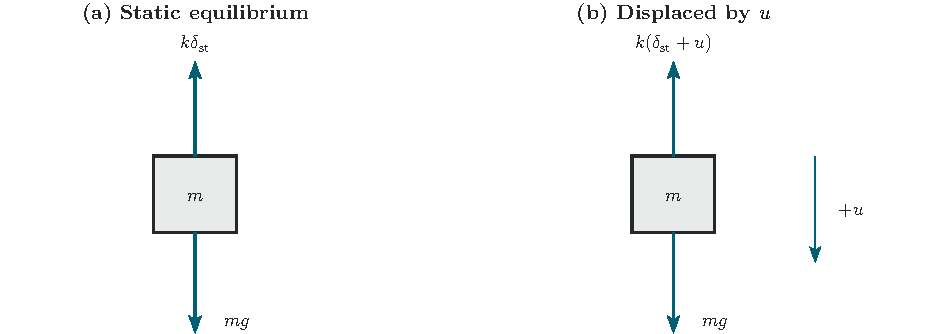
\includegraphics[width=0.95\linewidth,height=0.30\textheight,keepaspectratio,alt={Free-body diagrams for static equilibrium and vertical vibration in Problem C.1.}]{figures/generated/solutions/vertical_fbd.pdf}
\caption{C.1.1.b and C.1.2.a. Free-body diagrams for static equilibrium and vertical vibration.}
\end{figure}

\textbf{C.1.1(c). Static equilibrium equation.} At equilibrium the acceleration is zero, so the downward weight and upward spring force balance. With downward positive,

\[
\sum F_y=mg-k\delta_{\mathrm{st}}=0.
\]

\[
\boxed{mg-k\delta_{\mathrm{st}}=0}
\qquad\text{(C.1.1.c)}
\]

\textbf{C.1.1(d). Static displacement.} Rearranging the equilibrium equation gives

\[
\delta_{\mathrm{st}}=\frac{mg}{k}.
\]

\[
\boxed{\delta_{\mathrm{st}}=\frac{mg}{k}}
\qquad\text{(C.1.1.d)}
\]

\textbf{C.1.2(b). Equation of motion.} Since \(u(t)\) is measured from static equilibrium, the absolute downward position is

\[
y(t)=\delta_{\mathrm{st}}+u(t).
\]

Because the spring deformation is \(\delta_{\mathrm{st}}+u(t)\), the net vertical force is

\[
\sum F_y=mg-k\bigl(\delta_{\mathrm{st}}+u(t)\bigr)
 =\bigl(mg-k\delta_{\mathrm{st}}\bigr)-ku(t).
\]

The first parenthesis is zero from static equilibrium. Newton's law therefore gives

\[
m\ddot{u}(t)=\sum F_y=-ku(t),
\]

which becomes the homogeneous free-vibration equation

\[
\boxed{m\ddot{u}(t)+ku(t)=0}
\qquad\text{(C.1.2.b)}
\]

\textbf{C.1.2(c). Comparison with B.1.} The equation is the same as the horizontal spring-mass equation because the constant gravitational force is canceled by the static spring force. Gravity changes the absolute equilibrium position through \(\delta_{\mathrm{st}}\), but it does not appear in the incremental vibration equation. Dividing by \(m\) gives

\[
\boxed{\ddot{u}(t)+\frac{k}{m}u(t)=0,
\qquad \omega_n=\sqrt{\frac{k}{m}}}
\qquad\text{(C.1.2.c)}
\]

\textbf{C.1.3. Arbitrary force field.} Let \(F(y,t)\) be the force magnitude and define its signed component along the downward coordinate by

\[
Q(y,t)=F(y,t)\cos\theta(y,t).
\]

The absolute equation of motion becomes

\[
m\ddot{y}+ky=mg+Q(y,t).
\]

For a time-independent field, let \(y_e\) be the equilibrium position, so that \(ky_e=mg+Q(y_e)\). Setting \(y=y_e+u\) and subtracting the equilibrium equation gives

\[
m\ddot{u}+ku=Q(y_e+u)-Q(y_e).
\]

Thus, a constant force component only shifts the equilibrium and disappears from the incremental equation. A position-dependent field changes the effective stiffness. For small displacement, linearization gives

\[
Q(y_e+u)-Q(y_e)\approx Q'(y_e)u,
\]

so the linearized equation is

\[
\boxed{m\ddot{u}+\bigl[k-Q'(y_e)\bigr]u=0}
\qquad\text{(C.1.3)}
\]

If the field varies with time, its time-varying component remains as an external forcing term. A force component perpendicular to the allowed motion is handled by the constraint in this one-coordinate model; otherwise, an additional coordinate and a coupled equation are required.

\endgroup
